\newpage
\subsubsection{detectIslets}
\label{subsub:IMdetectIslets}
I denne funktion sker selve billedesegmenteringen af de langerhanske øer. Selve segmenteringen sker via en række morfologiske operationer, som er nærmere beskrevet i dette afsnit. For at illustrere effekten af de enkelte steps er der i løbet af afsnittet vist billeder.

I figur \ref{fig:im} er det oprindelige billede vist. Billedet danner udgangspunktet for selve segmenteringen. Billedet indeholder én langerhansk ø. 

%\begin{lstlisting} 
% Converts the image to logical, based on threshold. 0.72 indicates pixels
% with luminance level above 0,72 (255*0.72 = 183) is converted to a 1. Pixels below this 
% level is converted to 0 
%bw = im2bw(im,0.72);
%\end{lstlisting} 

\begin{figure}[H]
	\centering
	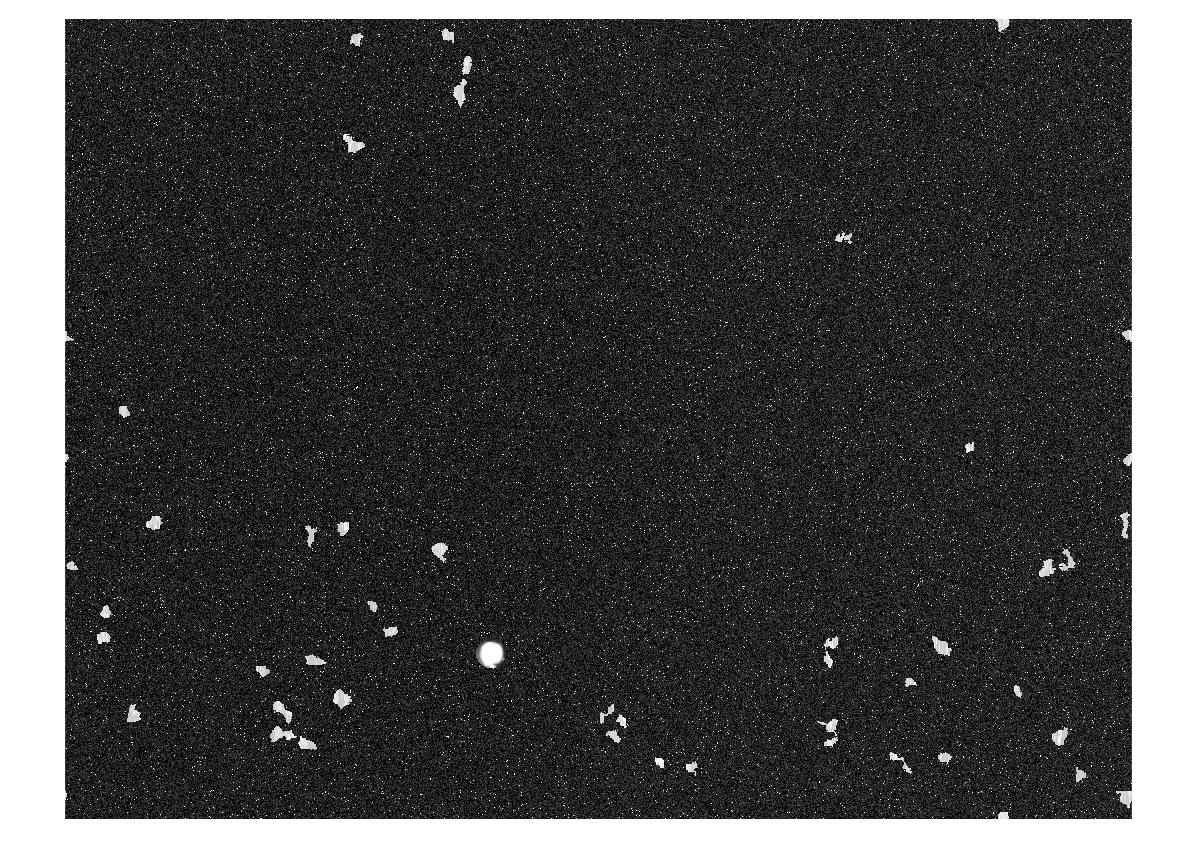
\includegraphics[width=0.6\textwidth]{billeder/software/im.png}
	\caption{Oprindelige billede}
	\label{fig:im}
\end{figure}

Første step af billedesegmenteringen består i, at konvertere det oprindelige billede (\ref{fig:im}) til en logisk maske. Til dette er Matlab funktionen \textit{im2bw} anvendt. 
Effekten af im2bw er vist i figur \ref{fig:im2bw}. Funktionen konvertere alle pixels med en lysstyrke over det angivne threshold (0,72) med 1, og pixels under med 0. Input billedet er et 8 bit billede, dermed indikerer et threshold på 0,72, at pixel værdien skal være over 183 for at blive inkluderet i masken. I nedenstående kode er implementeringen vist.

\begin{lstlisting} 
% Converts the image to logical, based on threshold. 0.72 indicates pixels
% with luminance level above 0,72 (255*0.72 = 183) is converted to 1. Pixels below this 
% level is converted to 0 
bw = im2bw(im,0.72);
\end{lstlisting} 

\begin{figure}[H]
	\centering
	
\includegraphics[width=0.6\textwidth]{billeder/software/im2bw.png}
	\caption{Billede konverteret til logisk}
	\label{fig:im2bw}
\end{figure}

I næste step bliver unødigt støj fra masken fjernet. Til dette anvendes funktionen \textit{bwareaopen}. Denne fjerner alle objekter i masken under 100 sammenhørende px. Dette fjerner de mindste støjkomponenter fra billedet. Effekten af denne funktion er vist i figur \ref{fig:bwarea}. Herudover kaldes funktionen bwlabel, som indeksere hvert af de sammenhørende objekter i masken. Dermed får hvert objekt i figur \ref{fig:bwarea} et unikt index fra 1 til 5. 
\begin{lstlisting} 
% Removes all objects below 100 connected pixels
bw = bwareaopen(bw,100);

% Label connected components
L = bwlabel(bw);
\end{lstlisting} 

\begin{figure}[H]
	\centering
	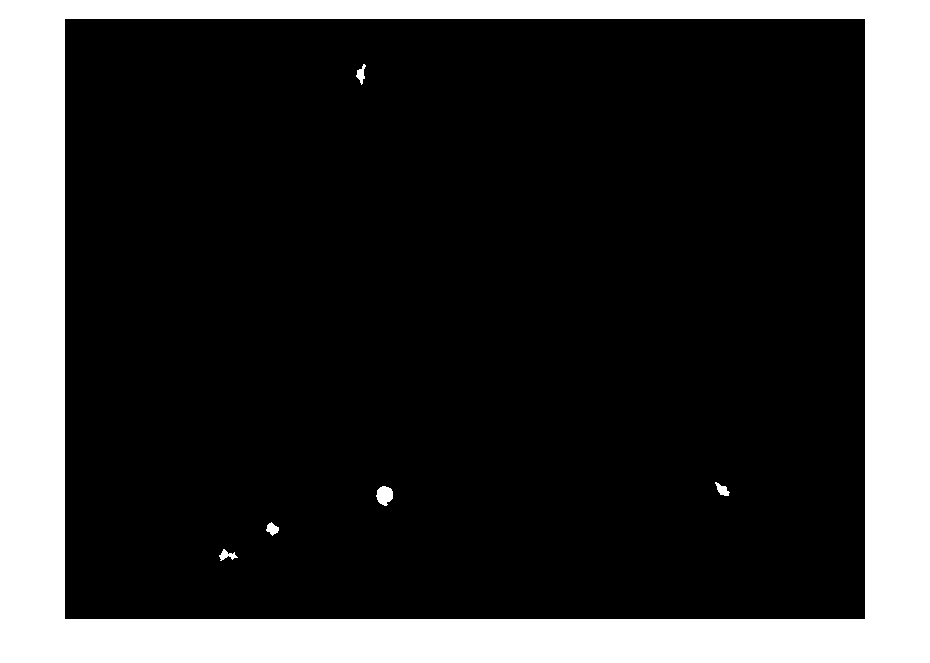
\includegraphics[width=0.6\textwidth]{billeder/software/bwarea.png}
	\caption{Små objekter fjernet}
	\label{fig:bwarea}
\end{figure}

I næste step sker selve ø detekteringen. Detektionen baseres på, at øerne har en mere cirkulær form end resten af vævet. Derfor hentes der egenskaber fra objekterne i masken vha. matlab funktionen \textit{regionsprops}. De egenskaber der hentes er med til, at beskrive hvor cirkulært objektet er. De egenskaber som hentes er arealet, center positionen, omkredsen og excentriciteten. Excentriciteten beskriver hvor langstrakt objektet er. Hvis excentriciteten er 0 er det en perfekt cirkel mens det vil være en langstrakt ellipse hvis værdien er 1.

Udfra arealet og omkredsen af objekterne anvendes de 2 nedenstående formler til bestemmelse af 2 værdier for radiusen af objektet:
\begin{align}
Areal = R1^2*\pi => R1 = \sqrt{\frac{\text{Areal}}{\pi}}
\end{align}
\begin{align}
Omkreds = 2*R2*\pi => R2 = \frac{\text{Omkreds}}{2*\pi}
\end{align}

Udfra disse 2 radius værdier, vil det objekt, hvor der er mindst forskel i mellem de 2, være det objekt der er mest cirkulært. Til at illustrere dette er der i figur \ref{fig:circleelip} vist en cirkel og en ellipse begge med samme areal. Udfra \textit{regionsprops} og de 2 formler for radius kan der bestemmes 2 radiuser for henholdsvis cirklen og ellipsen. Forskellen bestemmes ved, at trække de 2 beregnede værdier fra hinanden. I udregningerne nedenfor er den første kolonne værdier for cirklen, mens den anden er for ellipsen. Som det ses er forskellen mindst ved cirklen, hvilket indikerer, at den er mest cirkulær.
  
\begin{lstlisting} 
r1 =  100.0017   99.9380

r2 =  99.7978  105.7890

rDif = 0.2039    5.8510
\end{lstlisting} 

\begin{figure}[H]
	\centering
	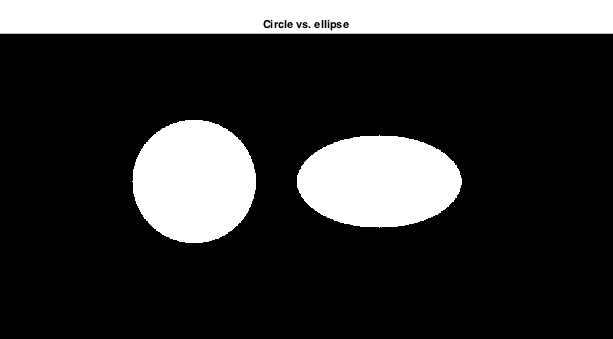
\includegraphics[width=0.6\textwidth]{billeder/software/circleellipse.png}
	\caption{Cirkel sammenlignet med ellipse}
	\label{fig:circleelip}
\end{figure}

Indekset for det objekt med mindst forskel i radius og indekset for det objekt med den mindste excentricitet gemmes i variabler. I nedenstående kode er det vist, hvordan dette er implemeneteret i Matlab.

\begin{lstlisting} 
stats = regionprops(bw,'Area','Centroid','Perimeter','Eccentricity');

r1 = sqrt([stats.Area]/pi);
r2 = [stats.Perimeter]/(2*pi);
% The absolute difference between the 2 radius is calculated
rDif = abs(r1-r2);
% The index of the lowest difference is returned
[~, idx] = min(rDif);
% The index of the object with the lowest eccentricity is returned 
[~, idx2] = min([stats.Eccentricity]);
\end{lstlisting} 

I det sidste step i segmenteringen af den langerhanske ø kontrolleres det om radius forskellen og excentricitet ligger under nogle fast definerede grænseværdier. Værdierne er fundet ved, at analysere en række billeder og deres objekters radius og excentricitet. Radius og excentriciteten bliver gemt i logfilen, så de kan analyseres for senere at justere grænseværdierne. Hvis objektets værdier er under disse grænseværdier er en ø detekteret. Når en ø er detekteret illustreres det med en grøn ring på GUI. Til dette er funktionen \textit{viscircles} anvendt, hvor center positionen og radius for objektet anvendes. 

For at løse udfordringen med, at den samme ø vil optræde på det næste billede, er der implementeret et smalt detekteringsvindue (100 pixels bredt). Når øen er detekteret inden for dette område bliver variablen isletDetected sat til true. Denne variabel anvendes til styring af ventilen. Implementingen af dette er vist i nedenstående kode.


\begin{lstlisting} 
% If the difference between radius AND eccentricity is below the defined
 % values an islet has been detected
 if rDif(idx) < 0.45 && stats(idx2).Eccentricity <0.51
     
 % Show circle of cell on the 2 axes
 viscircles(h,stats(idx2).Centroid,r1(idx2)+10,...
 'LineStyle','-','edgecolor','g','LineWidth',1,'DrawBackgroundCircle',...
 false);
 viscircles(s,stats(idx2).Centroid,r1(idx2)+10,...
 'LineStyle','-','edgecolor','g','LineWidth',1,'DrawBackgroundCircle',...
 false);

     
      % Detection window  (0 to 100 pixels)
      if stats(idx2).Centroid(1) <=100 
      handles.flag1 = true;
      handles.count = handles.count+1; 
      set(handles.txtIslets,'String',num2str(handles.count));
      handles.isletDetected = true;
      end
\end{lstlisting} 

Figur \ref{fig:segmented} viser slutresultatet af segmenteringen, hvor masken kun indeholder den langerhanske ø fra det oprindelige billede. 


\begin{figure}[H]
	\centering
	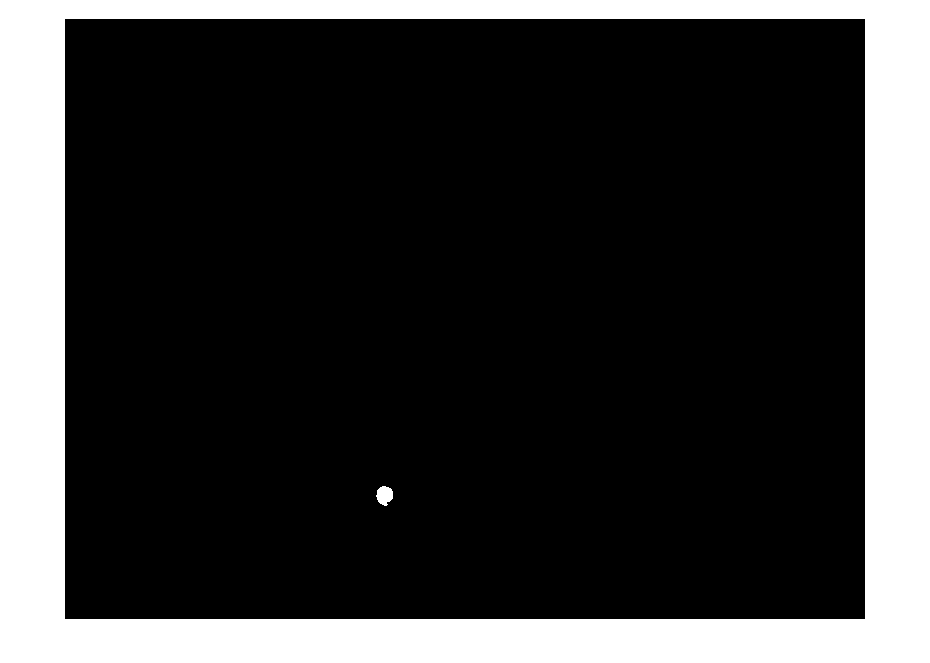
\includegraphics[width=0.6\textwidth]{billeder/software/segmented.png}
	\caption{Slutresultat af segmentering}
	\label{fig:segmented}
\end{figure}

I figur \ref{fig:finalimage} er det oprindelige billede vist, med markering af den detekterede ø.


\begin{figure}[H]
	\centering
	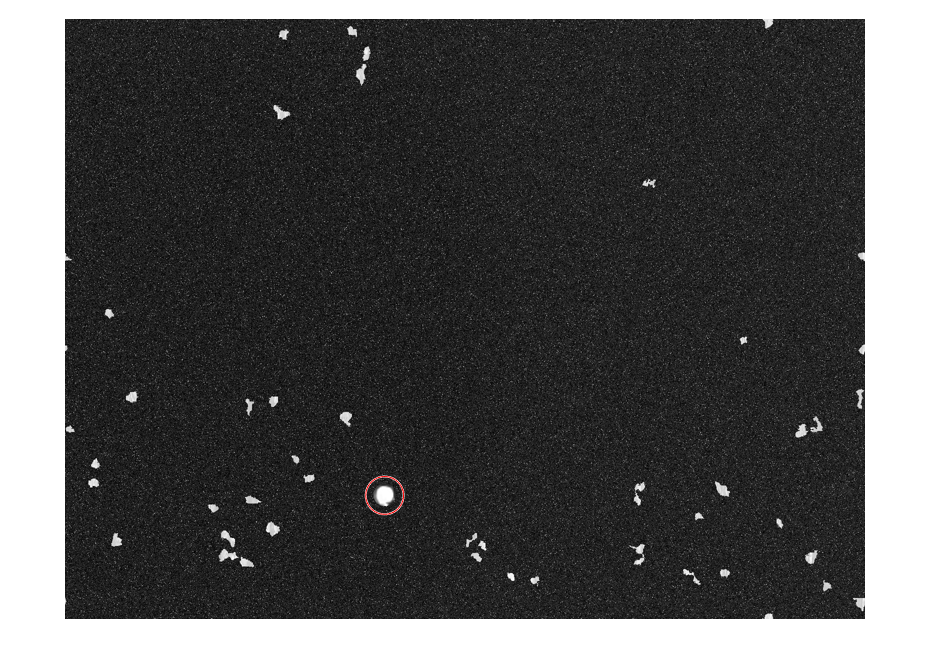
\includegraphics[width=0.6\textwidth]{billeder/software/finalimage.png}
	\caption{Oprindelige billede med detekteret ø}
	\label{fig:finalimage}
\end{figure}

\newpage
\textbf{Test af billedeprocessering}

En udfordring med billedeprocesseringen er, at hastigheden ikke må være for langsom i forhold til frameraten for kameraet. Som beskrevet under funktionen cameraFeed (\ref{subsub:camfeed} indlæses et nyt billede hvert 0,1 sekund. Billedeprocesseringen skal dermed være hurtigere end dette for at følge med. Til test af dette er Matlab funktionen tic/toc anvendt, som måler hvor langt tid billedprocessingen tager om at eksekvere. I figur \ref{fig:dataprocess} viser grafen hvor lang tid det har taget, at behandle de enkelte billeder. Den røde streg viser den gennemsnitlige tid for processeringen. For den nuværende implementering tager billedeprocessingen 0,0104 sekund pr. billede, hvilket er indenfor grænsen på 0,1 sekund. Tiden vil variere alt efter tilgængelig processorkraft og om der skal udføres andre opgaver, eksempelvis opdatere figurer på GUI. 

\begin{figure}[H]
	\centering
	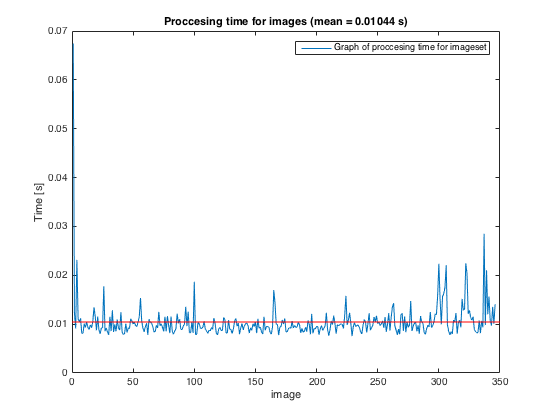
\includegraphics[width=0.6\textwidth]{billeder/software/dataprocessing_2.png}
	\caption{Test af tidsforbrug for billedeprocessering}
	\label{fig:dataprocess}
\end{figure}
